\documentclass[conference]{IEEEtran}
\usepackage[T1]{fontenc}
\usepackage{cite}
\usepackage{graphicx,amsmath,amssymb,booktabs,array,xurl}
\usepackage{tikz}
\usetikzlibrary{arrows.meta,positioning,calc,fit}
\usepackage[hidelinks]{hyperref}
\graphicspath{{figures/}}
\makeatletter\newcommand{\gen}[1]{\@@input generated/#1 }\makeatother
\definecolor{gat}{HTML}{2A78D6}
\definecolor{gru}{HTML}{EB6834}
\definecolor{ink}{HTML}{52514E}
\definecolor{resp}{HTML}{6250D6}

\title{Graph-Attention Traffic Speed Forecasting\\and a Synthetic LWR Signal-Control Study}
\author{\IEEEauthorblockN{Kavya Katal, Rudraksh Sharma, Anshuman Mehta, Vridhi Chaudhary, Bineet Keshari}
\IEEEauthorblockA{Team T072, Section C, Rishihood University\\
Project 4, Phase 2 (Deep Learning) report, November 2026}}

\begin{document}
\maketitle

\begin{abstract}
Phase 1 of this project forecast traffic speed on the METR-LA sensor network with one tree model per sensor. Phase 2 asks a narrower deep-learning question: does information from neighbouring sensors on the road graph improve a neural forecaster? We train a shared gated recurrent unit (GRU) and the same GRU followed by a graph-attention (GAT) layer under one chronological, leakage-controlled protocol, with three seeds and three ablations. At 60 minutes the GRU+GAT model reaches a test mean absolute error (MAE) of 4.881\,mph, against 4.931\,mph for an identical model restricted to self-loops and 4.929\,mph for the temporal GRU. The gain from neighbours is real but small, and it grows with the forecast horizon. Both neural models remain well behind the frozen Phase 1 XGBoost baseline (3.874\,mph), and a validation-selected XGBoost--GAT blend reduces to pure XGBoost, so we report no hybrid gain. A separate synthetic experiment implements Lighthill--Whitham--Richards (LWR) dynamics with a cell-transmission model and compares two local rule-based signal agents with a fixed-time plan. It is not calibrated to Los Angeles and is not driven by the forecasts. All forecasting scores are exploratory because the test interval was inspected during Phase 1.
\end{abstract}

\begin{IEEEkeywords}
traffic forecasting, METR-LA, gated recurrent unit, graph attention network, ablation study, cell transmission model
\end{IEEEkeywords}

\section{Introduction}
Road traffic is a spatio-temporal process. The speed at a loop detector depends on its own recent history and on conditions at connected locations, because queues spill back along a road and released traffic moves downstream. A forecaster that sees only one sensor ignores the second effect.

Phase 1 built such single-sensor forecasters. Its Random Forest and XGBoost models used 38 causal features computed from each sensor's own last 55 minutes and never looked at a neighbour. Phase 2 tests whether a deep model that can look at neighbours does better, and it is designed so that the answer can be attributed to the neighbours and not to some other change. The project title also names LWR traffic-flow models and multi-agent control, so a small simulation covers those two topics separately.

This report makes four contributions.
\begin{itemize}
\item A shared GRU encoder with an optional graph-attention layer, trained under the Phase 1 chronological protocol with training-only statistics and masked targets (Sections III--V).
\item A controlled comparison: the full model, a self-loop control, a uniform-weight control and a no-dropout control, with three seeds for the main comparison (Section VII).
\item An honest account of two negative results: the neural models do not beat the tree baselines, and the ML--DL blend selects pure XGBoost (Section VII).
\item A conservative eight-cell LWR/cell-transmission simulation with two local signal agents, kept separate from the forecasting study (Section VIII).
\end{itemize}

\section{Related Work}
\textbf{Recurrent sequence models.} Cho \emph{et al.} introduced the gated recurrent unit, whose reset and update gates let a recurrent network keep or overwrite its memory at each step \cite{cho}. We use it as the temporal encoder. Pascanu \emph{et al.} analysed exploding gradients in recurrent networks and proposed clipping the gradient norm \cite{pascanu}, which we apply.

\textbf{Graph neural networks.} Veli\v{c}kovi\'c \emph{et al.} proposed graph attention networks, in which a node aggregates its neighbours with weights computed by a small attention function and normalised by a masked softmax \cite{gat}. Our graph layer follows that additive formulation. Jain and Wallace showed that attention weights need not be faithful explanations of a model's output \cite{attn}; we therefore treat our attention weights as fitted behaviour, not as evidence of physical influence between roads.

\textbf{Spatio-temporal traffic forecasting.} Li \emph{et al.} modelled traffic as diffusion on a directed sensor graph inside an encoder--decoder recurrent network (DCRNN) and released the METR-LA benchmark and its sensor graph \cite{dcrnn}. Yu \emph{et al.} replaced recurrence with gated temporal convolutions between graph convolutions (STGCN) \cite{stgcn}. Wu \emph{et al.} added a learned adjacency matrix and dilated convolutions (Graph WaveNet) \cite{gwn}. These systems are far larger than ours and use different splits and training procedures, so we do not rank our scores against their published numbers. Our model is a deliberately small GRU with one attention layer, built to isolate one question.

\textbf{Traffic-flow theory.} Lighthill and Whitham \cite{lw} and Richards \cite{richards} described traffic as a conserved density whose flow depends on density, which gives the LWR kinematic-wave model. Daganzo's cell transmission model (CTM) discretises it with sending and receiving limits per cell \cite{ctm1} and extends it to networks \cite{ctm2}. We implemented the update from the Berkeley PATH technical overview \cite{ctmoverview}.

\textbf{Signal control.} Varaiya's max-pressure controller chooses the phase with the largest upstream-minus-downstream queue using only local measurements, and comes with a stability guarantee for a store-and-forward network \cite{maxpressure}; Lioris and Varaiya study decentralised variants \cite{lioris}. Our responsive agent borrows the local pressure idea only. It uses cell occupancy, adds minimum and maximum green times, and inherits no guarantee.

\textbf{Baselines.} The Phase 1 comparators are Random Forest \cite{rf} and XGBoost \cite{xgb}.

\section{Data and Preparation}
\subsection{Dataset}
METR-LA contains speed readings from 207 loop detectors on Los Angeles County highways, every five minutes from 1 March to 27 June 2012: 34,272 time steps \cite{dcrnn}. Speeds are in miles per hour. The file records no time zone. The benchmark stores missing readings as zero; we treat zero and NaN as missing, which covers 8.11\% of all readings and 7.13\% of the training interval. The sensor graph is the directed, thresholded Gaussian-kernel adjacency distributed with DCRNN, with 1,515 directed edges between distinct sensors. Our rebuilt adjacency matches the distributed one.

\subsection{Windows and splits}
Each sample uses the 12 readings up to the forecast origin $t$ (55 minutes) to predict the next 12 readings (5 to 60 minutes ahead). We report the 15-, 30- and 60-minute horizons. Origins are split in time order into 23,963 training, 1,701 tuning-validation, 1,702 reserved-validation and 6,850 test origins. Eleven origins are removed before each boundary so that no target of one part falls inside the next part. Training uses every second origin; evaluation uses every origin.

\subsection{Leakage controls}
Every statistic is fitted on valid training readings only: one global mean and standard deviation for normalisation and one median per sensor for filling. Inside a history window a missing reading is filled forward from an earlier reading in the same window, and a leading gap takes the sensor's training median. Nothing is filled backward. The original missing flag is kept as a second input channel. Targets are never filled: a missing target is excluded from the loss and from every metric by a mask shared by all methods.

\subsection{Model inputs}
The network input has shape $B\times12\times207\times2$ (normalised speed and missing flag). Five calendar values of the origin (sine and cosine of time of day and of day of week, and a weekend flag) are given to the output layer. The output has shape $B\times12\times207$.

\section{Model Architecture}
\begin{figure*}[t]
\centering
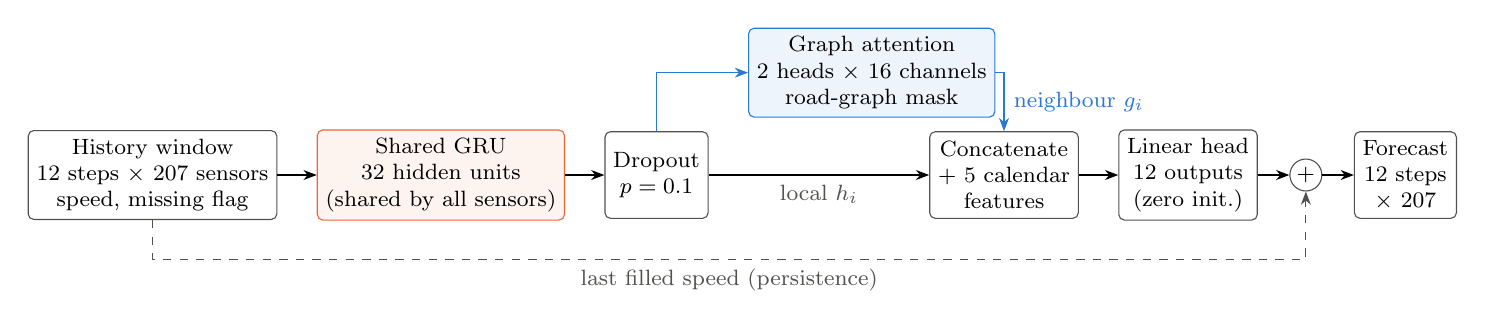
\begin{tikzpicture}[font=\footnotesize, >=Stealth,
  box/.style={draw=ink, rounded corners=2pt, align=center, minimum height=11mm, inner sep=3pt, fill=white},
  gbox/.style={box, draw=gat, fill=gat!8},
  ebox/.style={box, draw=gru, fill=gru!8}]
\node[box] (in) {History window\\$12$ steps $\times$ $207$ sensors\\speed, missing flag};
\node[ebox, right=5mm of in] (gru) {Shared GRU\\32 hidden units\\(shared by all sensors)};
\node[box, right=5mm of gru] (drop) {Dropout\\$p=0.1$};
\node[gbox, right=5mm of drop, yshift=13mm] (gat) {Graph attention\\2 heads $\times$ 16 channels\\road-graph mask};
\node[box, right=28mm of drop] (cat) {Concatenate\\+ 5 calendar\\features};
\node[box, right=5mm of cat] (head) {Linear head\\12 outputs\\(zero init.)};
\node[circle, draw=ink, inner sep=1pt, right=4mm of head] (sum) {$+$};
\node[box, right=4mm of sum] (out) {Forecast\\12 steps\\$\times$ 207};
\draw[->] (in) -- (gru);
\draw[->] (gru) -- (drop);
\draw[->] (drop) -- node[below, text=ink]{local $h_i$} (cat);
\draw[->, gat] (drop.north) |- (gat.west);
\draw[->, gat] (gat.east) -| node[pos=0.75, right, text=gat]{neighbour $g_i$} (cat.north);
\draw[->] (cat) -- (head);
\draw[->] (head) -- (sum);
\draw[->] (sum) -- (out);
\draw[->, ink, dashed] (in.south) -- ++(0,-5mm) -| node[pos=0.25, below, text=ink]{last filled speed (persistence)} (sum.south);
\end{tikzpicture}
\caption{Model. The temporal GRU uses the black path only. GRU+GAT adds the blue branch, in which each sensor attends to the sensors allowed by the road graph. The head predicts a correction to the last observed speed, so an untrained model equals the persistence forecast.}
\label{fig:arch}
\end{figure*}

Fig.~\ref{fig:arch} shows both models. They share every component except the blue branch.

\subsection{Shared temporal encoder}
One single-layer GRU with 32 hidden units reads each sensor's 12-step window. The same weights are used for all 207 sensors, which keeps the model small and lets every sensor's data train the same encoder. With input $x_t$, previous state $h_{t-1}$, sigmoid $\sigma$ and element-wise product $\odot$, the PyTorch GRU computes \cite{cho,torchgru}
\begin{align}
r_t&=\sigma(W_r x_t+U_r h_{t-1}+b_r),\\
z_t&=\sigma(W_z x_t+U_z h_{t-1}+b_z),\\
n_t&=\tanh\bigl(W_n x_t+b_n+r_t\odot(U_n h_{t-1}+c_n)\bigr),\\
h_t&=(1-z_t)\odot n_t+z_t\odot h_{t-1}.
\end{align}
The reset gate $r_t$ decides how much past state enters the candidate $n_t$, and the update gate $z_t$ decides how much of the old state is kept. The state starts at zero for every window. The final state $h_i\in\mathbb{R}^{32}$ summarises sensor $i$.

\subsection{Graph-attention layer}
The graph model passes the 207 summaries through one attention layer with $K=2$ heads of 16 channels \cite{gat}. For head $k$, with projection $W$ and attention vectors $a_r^{k},a_s^{k}$,
\begin{align}
e_{ij}^{k}&=\operatorname{LeakyReLU}\bigl(a_r^{k\top}Wh_i+a_s^{k\top}Wh_j\bigr),\\
\alpha_{ij}^{k}&=\frac{\exp(e_{ij}^{k})}{\sum_{l\in\mathcal N_i}\exp(e_{il}^{k})},\\
g_i&=\operatorname{ELU}\Bigl(\bigl\Vert_{k=1}^{K}\sum_{j\in\mathcal N_i}\alpha_{ij}^{k}\,Wh_j\Bigr),
\end{align}
where $\Vert$ concatenates the heads. The neighbourhood $\mathcal N_i$ contains sensor $i$ and every sensor $j$ with a graph edge from $j$ to $i$. The Gaussian edge weights decide only who is a neighbour; the attention weights are learned. Whether an edge is physically upstream or downstream was not verified.

\subsection{Residual output}
The head is one linear layer on the concatenation of $h_i$, $g_i$ (graph model only) and the calendar vector $c_t$:
\begin{equation}
\hat y_{i,t+1:t+12}=\tilde x_{i,t}\,\mathbf 1+W_o\,[h_i;g_i;c_t]+b_o ,
\end{equation}
where $\tilde x_{i,t}$ is the last filled, normalised speed. $W_o$ and $b_o$ start at zero, so training starts from the persistence forecast and learns a correction to it. All 12 horizons are predicted in one step, not recursively.

\subsection{Design rationale}
The model is small on purpose: 3,912 parameters for the temporal GRU and 5,384 for GRU+GAT. A small model trains in minutes on a laptop CPU, which made three seeds and several ablations affordable, and it keeps the comparison between variants clean. The cost of this choice is accuracy, as Section VII shows.

\section{Training and Regularisation}
\subsection{Objective and optimiser}
The loss is the mean absolute error over valid targets in normalised units,
\begin{equation}
\mathcal L=\frac{1}{|\mathcal M|}\sum_{(i,h)\in\mathcal M}\bigl|\hat y_{i,h}-y_{i,h}\bigr|,
\end{equation}
where $\mathcal M$ is the set of non-missing targets in the batch. We use Adam \cite{adam}. Table~\ref{tab:hyper} lists all settings, fixed in a configuration file before any real-data training.

\begin{table}[t]\centering\small
\caption{Training settings, fixed before training.}\label{tab:hyper}
\begin{tabular}{@{}ll@{}}\toprule
Setting & Value\\\midrule
History / horizon & 12 / 12 steps (5\,min each)\\
GRU hidden units & 32, one layer\\
Attention & 2 heads $\times$ 16 channels\\
Loss & masked MAE (normalised)\\
Optimiser & Adam, weight decay $10^{-4}$\\
Learning rates tried & $10^{-3}$, $3\times10^{-4}$\\
Batch size & 32 origins (all 207 sensors)\\
Dropout & 0.1 on embeddings and attention\\
Gradient clipping & norm 5\\
Epochs & at most 50, patience 7\\
Seeds & 42, 43, 44\\
Device & CPU, PyTorch 2.7.1\\
\bottomrule\end{tabular}
\end{table}

\subsection{Regularisation}
Four mechanisms limit over-fitting and unstable training. Dropout \cite{dropout} with $p=0.1$ is applied to the GRU summaries and to the attention weights. A one-layer GRU has no between-layer dropout, so this is added explicitly. Weight decay of $10^{-4}$ penalises large weights. The gradient norm is clipped at 5 \cite{pascanu}. Early stopping ends a run after seven epochs without improvement on the tuning-validation set and keeps the checkpoint of the best epoch. Weight sharing across sensors acts as a fifth, structural regulariser.

\subsection{Learning-rate selection}
For each family we trained seed 42 with both learning rates and chose the rate with the lower tuning-validation MAE averaged over the three headline horizons (Table~\ref{tab:tune}). The rate $10^{-3}$ won in both families. Fig.~\ref{fig:learning} shows the validation curves of the two selected runs. No setting was chosen using test scores.

\begin{table}[t]\centering\small
\caption{Learning-rate search on tuning validation (seed 42). MAE is the mean over 15, 30 and 60 minutes, in mph.}\label{tab:tune}
\begin{tabular}{@{}lrrrc@{}}\toprule
Family & Rate & Val.\ MAE & Epochs & Chosen\\\midrule
\gen{table_tuning.tex}
\bottomrule\end{tabular}
\end{table}

\begin{figure}[t]\centering
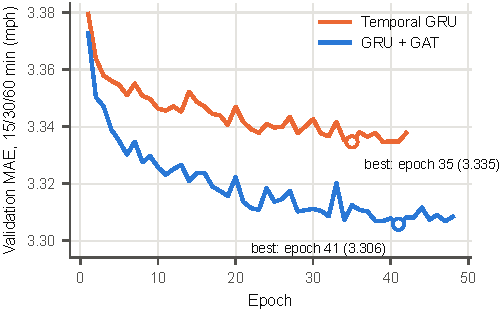
\includegraphics[width=\columnwidth]{learning.pdf}
\caption{Tuning-validation MAE per epoch for the two selected seed-42 runs. Circles mark the checkpoint kept by early stopping.}\label{fig:learning}
\end{figure}

\section{Experimental Design}
\subsection{Compared methods}
The references are the four frozen Phase 1 methods: persistence (repeat the last reading), historical average (training mean by sensor and time of week), Random Forest and XGBoost. Their saved predictions were re-scored on the same targets and reproduce all recorded Phase 1 metric rows. The neural methods are the temporal GRU and GRU+GAT.

\subsection{Ablations}
Three controls change one thing in the graph model and keep its tuned settings.
\begin{itemize}
\item \emph{Self-loop only}: the neighbourhood is reduced to the sensor itself. The layer and its parameter count stay; only neighbour access is removed.
\item \emph{Uniform neighbours}: the same neighbours are averaged with equal weights. This removes the learned weighting.
\item \emph{No dropout}: dropout is set to zero.
\end{itemize}
The temporal GRU also lacks neighbours, but it is a smaller model, so the self-loop control is the fair test of neighbour access. The main models and the self-loop control use three seeds. The other two controls use seed 42 only.

\subsection{Hybrid}
The optional hybrid is a blend $\hat y=\lambda\,\hat y_{\mathrm{XGB}}+(1-\lambda)\,\hat y_{\mathrm{GAT}}$ with one global weight $\lambda\in\{0,0.25,0.5,0.75,1\}$. The weight is chosen on the reserved-validation set, which no base model used for tuning, and is frozen before the test set is scored. The rationale is that trees and a graph network make different errors, so an average could beat both. The two pure models are included as candidates, so the procedure can also report that blending does not help.

\subsection{Metrics}
With $e_j=\hat y_j-y_j$ over the $n$ valid targets of a horizon,
\begin{align}
\mathrm{MAE}&=\frac1n\sum_j|e_j|,\qquad
\mathrm{RMSE}=\sqrt{\frac1n\sum_j e_j^2}.
\end{align}
Both are in mph and lower is better. RMSE weights large misses more heavily. The test set gives about 1.25 million valid targets per horizon; overlapping forecasts are dependent, so this is not the number of independent trials.

\section{Results}
\subsection{Main comparison}
\begin{table*}[t]\centering\small
\caption{Test error in mph (exploratory test interval). Neural rows are the mean $\pm$ sample standard deviation over three separately trained seeds. Phase 1 rows are frozen single runs. Bold marks the lowest value in a column.}\label{tab:main}
\begin{tabular}{@{}lrrrrrr@{}}\toprule
Method & MAE 15\,min & MAE 30\,min & MAE 60\,min & RMSE 15\,min & RMSE 30\,min & RMSE 60\,min\\\midrule
\gen{table_main.tex}
\bottomrule\end{tabular}
\end{table*}

\begin{figure*}[t]\centering
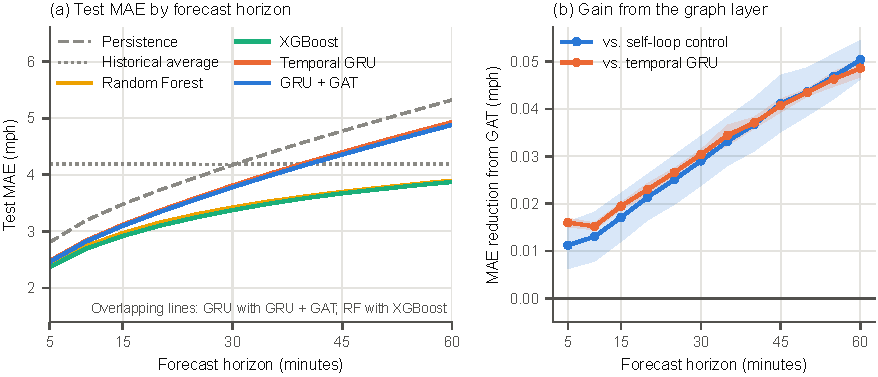
\includegraphics[width=\textwidth]{horizons.pdf}
\caption{(a) Test MAE at every horizon. (b) MAE reduction of GRU+GAT relative to its self-loop control and to the temporal GRU, as the mean of per-seed differences; bands show $\pm$ one sample standard deviation over three seeds.}\label{fig:horizons}
\end{figure*}

Table~\ref{tab:main} and Fig.~\ref{fig:horizons}(a) give three findings.

First, both neural models beat persistence at every horizon. GRU+GAT lowers persistence MAE by 11.0\% at 15 minutes and 8.3\% at 60 minutes.

Second, the tree baselines are clearly better. XGBoost has the lowest MAE at every headline horizon and Random Forest the lowest RMSE. At 60 minutes GRU+GAT is 1.007\,mph (26.0\%) above XGBoost.

Third, from 40 minutes (temporal GRU) or 45 minutes (GRU+GAT) onward the neural models are also worse than the historical average (4.187\,mph), which uses no recent reading at all. The neural correction to persistence is too weak at long horizons, where the typical speed for that time of week is the better guide.

A likely reason for the gap, which we did not test, is model form. Phase 1 fits a separate model for every sensor, so each model can learn that sensor's own daily pattern from the clock features. Our network shares all weights and has no sensor-specific input, so it must describe 207 different roads with 5,384 parameters.

\subsection{Does the graph help?}
\begin{table}[t]\centering\small
\caption{Ablations: test MAE in mph and change at 60\,min relative to the full model. Positive change means worse. Three-seed rows are means; their sample standard deviations are at most 0.007\,mph (Table~\ref{tab:main}, Fig.~\ref{fig:abl}).}\label{tab:abl}
\setlength{\tabcolsep}{3.5pt}
\begin{tabular}{@{}lrrrr@{}}\toprule
Variant & 15\,min & 30\,min & 60\,min & $\Delta_{60}$\\\midrule
\multicolumn{5}{@{}l}{\emph{Seed 42}}\\
\gen{table_ablation.tex}
\bottomrule\end{tabular}
\end{table}

\begin{figure}[t]\centering
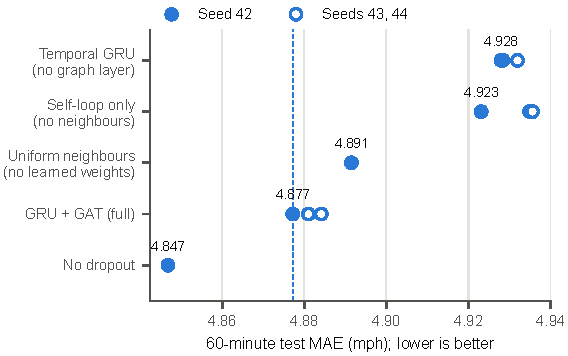
\includegraphics[width=\columnwidth]{ablation.pdf}
\caption{60-minute test MAE of every trained variant and seed. The dashed line marks the full model at seed 42. Note the narrow axis: the whole range is 0.09\,mph.}\label{fig:abl}
\end{figure}

Yes, by a small margin. Over three seeds the full model has a 60-minute MAE of 4.881\,mph against 4.931\,mph for the self-loop control (Table~\ref{tab:abl}). The difference of 0.050\,mph is about 1\% and is several times the seed-to-seed spread, and the full model is better in all three seeds (Fig.~\ref{fig:abl}). Fig.~\ref{fig:horizons}(b) shows that the gain rises steadily from 0.011\,mph at 5 minutes to 0.050\,mph at 60 minutes. This pattern is what one would expect if neighbours carry information about traffic that has not yet reached the sensor, but the experiment does not prove that mechanism. Three seeds show run-to-run variation; they are not a significance test.

The self-loop control and the temporal GRU score almost the same (4.931 and 4.929\,mph). The extra layer and parameters alone therefore bring nothing; the gain comes from neighbour access.

\emph{Learned weights.} With equal weights the seed-42 MAE is 4.891\,mph. Of the 0.046\,mph seed-42 gain over the self-loop control, about 0.032 comes from simply averaging neighbours and 0.014 from learning the weights. This rests on one seed.

\emph{Dropout.} Removing dropout improved the seed-42 model by 0.030\,mph. For a model this small, dropout at 0.1 costs more than it protects. We kept the predeclared setting and did not retune after seeing this test result. It also rests on one seed.

\emph{Where the graph helps.} At the sensor level (seed 42), the full model is better than the self-loop control at 168 of 207 sensors and worse at 39, with a median gain of 0.049\,mph (Fig.~\ref{fig:map}). Most of the larger gains lie along the long corridors.

\begin{figure}[t]\centering
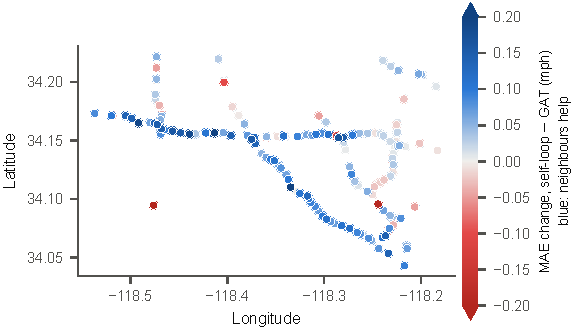
\includegraphics[width=\columnwidth]{sensor_map.pdf}
\caption{Per-sensor change in 60-minute MAE when neighbours are available (seed 42), at the sensor locations. Blue: GRU+GAT is better than its self-loop control. Red: worse.}\label{fig:map}
\end{figure}

\subsection{Traffic periods}
\begin{table}[t]\centering\small
\caption{60-minute test MAE by target period, mph. Peak is weekdays 07:00--10:00 and 16:00--19:00 in recorded clock time.}\label{tab:slices}
\setlength{\tabcolsep}{4pt}
\begin{tabular}{@{}lrrrr@{}}\toprule
Method & Peak & Off-peak & Weekday & Weekend\\\midrule
\gen{table_slices.tex}
\bottomrule\end{tabular}
\end{table}
Every method is much worse in peak periods (Table~\ref{tab:slices}). The neural models are closest to the trees at weekends, when traffic is smooth and persistence-like forecasts work, and furthest in peaks, when speeds change quickly. Random Forest, not XGBoost, is best in peaks.

\subsection{Hybrid result}
\begin{table}[t]\centering\small
\caption{Blend selection on reserved validation. MAE is the mean over 15, 30 and 60 minutes, in mph.}\label{tab:hybrid}
\begin{tabular}{@{}rrrc@{}}\toprule
XGBoost $\lambda$ & GAT $1-\lambda$ & Val.\ MAE & Chosen\\\midrule
\gen{table_hybrid.tex}
\bottomrule\end{tabular}
\end{table}
Validation error falls steadily as the XGBoost weight rises, and the best candidate is $\lambda=1$ (Table~\ref{tab:hybrid}). The selected ``blend'' is therefore pure XGBoost, and its test MAE equals the XGBoost row of Table~\ref{tab:main}. The hybrid was implemented and evaluated as planned, but it showed no value: the graph model is too far behind for its errors to help. We claim no hybrid improvement.

\subsection{Cost and output validity}
\begin{table}[t]\centering\small
\caption{Model size and recorded training cost. Minutes are mean wall-clock time per fit on a shared CPU and are not a clean speed benchmark.}\label{tab:cost}
\setlength{\tabcolsep}{4pt}
\begin{tabular}{@{}lrrrr@{}}\toprule
Variant & Params & Fits & Epochs & Min/fit\\\midrule
\gen{table_cost.tex}
\bottomrule\end{tabular}
\end{table}
Table~\ref{tab:cost} gives the model sizes and training times. None of the eleven evaluated fits produced a negative speed among its 17,015,400 raw test outputs, and no output was clipped. The output layer is unconstrained, so this is an observation about this data, not a guarantee.

\section{Synthetic LWR and Two-Agent Control}
This section is a separate experiment. METR-LA contains speed only: no density, flow or signal data. A physics model can therefore not be calibrated to it, and we do not convert forecast speeds into invented densities. The simulation below uses assumed parameters and invented demand.

\subsection{LWR and the cell-transmission update}
LWR conserves vehicles along a road \cite{lw,richards}:
\begin{equation}
\frac{\partial\rho}{\partial t}+\frac{\partial q}{\partial x}=0,\qquad q=\rho v,
\end{equation}
with density $\rho$ (veh/km), flow $q$ (veh/h) and speed $v$ (km/h). We use a triangular flow--density relation with free speed $v_f=60$\,km/h, backward wave speed $w=20$\,km/h and jam density $\rho_J=150$\,veh/km. Its capacity is $Q=v_f w\rho_J/(v_f+w)=2250$\,veh/h. The CTM \cite{ctm1,ctmoverview} divides the road into cells and limits each flow by what the upstream cell can send and what the downstream cell can receive:
\begin{align}
D_i&=\min(v_f\rho_i,\;Q),\qquad S_i=\min\bigl(Q,\;w(\rho_J-\rho_i)\bigr),\\
f_{i\to j}&=\begin{cases}\min(D_i,S_j)&\text{if the movement has green,}\\0&\text{otherwise,}\end{cases}\\
\rho_i^{k+1}&=\rho_i^{k}+\frac{\Delta t}{\Delta x}\bigl(f_{\mathrm{in}}-f_{\mathrm{out}}\bigr).
\end{align}
All flows are computed from the old state and applied together. With $\Delta x=0.25$\,km and $\Delta t=5$\,s, a vehicle at free speed covers 83\,m per step, less than one cell, which satisfies the CFL stability condition $\max(v_f,w)\,\Delta t/\Delta x\le1$. A cell stores at most 37.5 vehicles. Fractional vehicles are normal in a continuum model.

\begin{figure}[t]\centering
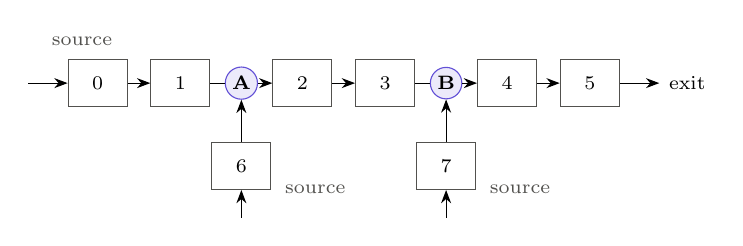
\begin{tikzpicture}[font=\scriptsize, >=Stealth,
  cell/.style={draw=ink, minimum width=7.5mm, minimum height=6mm, inner sep=0pt},
  sig/.style={circle, draw=resp, fill=resp!12, inner sep=1.2pt, font=\scriptsize\bfseries}]
\foreach \i/\x in {0/0,1/1.05,2/2.6,3/3.65,4/5.2,5/6.25} \node[cell] (c\i) at (\x,0) {\i};
\foreach \i/\j in {0/1,2/3,4/5} \draw[->] (c\i) -- (c\j);
\node[sig] (A) at ($(c1)!0.5!(c2)$) {A};
\node[sig] (B) at ($(c3)!0.5!(c4)$) {B};
\draw (c1) -- (A); \draw[->] (A) -- (c2);
\draw (c3) -- (B); \draw[->] (B) -- (c4);
\node[cell] (c6) at ($(A)+(0,-1.05)$) {6};
\node[cell] (c7) at ($(B)+(0,-1.05)$) {7};
\draw[->] (c6) -- (A); \draw[->] (c7) -- (B);
\draw[->] ($(c0.west)+(-5mm,0)$) -- (c0.west);
\draw[->] ($(c6.south)+(0,-3.5mm)$) -- (c6.south);
\draw[->] ($(c7.south)+(0,-3.5mm)$) -- (c7.south);
\draw[->] (c5.east) -- ++(5mm,0) node[right]{exit};
\node[anchor=south, text=ink] at ($(c0.north)+(-2mm,0.5mm)$) {source};
\node[anchor=west, text=ink] at ($(c6.east)+(0.5mm,-3mm)$) {source};
\node[anchor=west, text=ink] at ($(c7.east)+(0.5mm,-3mm)$) {source};
\end{tikzpicture}
\caption{Synthetic corridor: six main cells, two side cells, three source queues. Signal agent A lets either cell 1 or cell 6 enter cell 2; agent B lets either cell 3 or cell 7 enter cell 4.}\label{fig:corridor}
\end{figure}

\subsection{Network and agents}
Fig.~\ref{fig:corridor} shows the network. Arrivals wait in a source queue when the first cell is full, so no vehicle is dropped. Each signal agent serves one of two competing movements; during a 5-second all-red clearance neither moves.

The \emph{fixed-time} baseline repeats 40\,s main green, 5\,s all-red, 40\,s side green, 5\,s all-red, with agent B offset by 45\,s. The \emph{responsive} agent observes only the vehicle counts of its two approach cells and its downstream cell. Its pressure for an approach is $\max(n_{\mathrm{approach}}-n_{\mathrm{downstream}},0)$. After at least 20\,s of green it switches if the other approach's pressure is higher by more than 2 vehicles, or if its own approach is empty and the other is not; it must switch after 60\,s. The two agents exchange no messages. They influence each other only through the traffic between them. Both are hand-written rules. Nothing is learned, and the counts include moving vehicles, not only queued ones.

\subsection{Protocol}
Four scenarios were declared before any run: balanced demand, an arterial peak, a side-road peak and a 15-minute reduction of exit capacity. Each has 60 minutes of Poisson arrivals and 20 minutes of drain. Five seeds give 20 scenario--seed pairs, and both policies receive identical arrivals within a pair: 40 runs. No policy parameter was tuned on outcomes.

\subsection{Results}
\begin{table*}[t]\centering\small
\caption{Synthetic control results, mean over five paired seeds. System time counts all vehicles in cells and source queues; boundary wait counts source queues only. Both are vehicle-minutes. Reduction is the mean of the five paired reductions. These are simulation outputs, not Los Angeles measurements.}\label{tab:control}
\setlength{\tabcolsep}{4.5pt}
\begin{tabular}{@{}lrrrrrrr@{}}\toprule
 & \multicolumn{3}{c}{System time} & \multicolumn{2}{c}{Boundary wait} & \multicolumn{2}{c}{Vehicles left at end}\\\cmidrule(lr){2-4}\cmidrule(lr){5-6}\cmidrule(l){7-8}
Scenario & Fixed & Responsive & Red.\ (\%) & Fixed & Responsive & Fixed & Responsive\\\midrule
\gen{table_control.tex}
\bottomrule\end{tabular}
\end{table*}

\begin{figure}[t]\centering
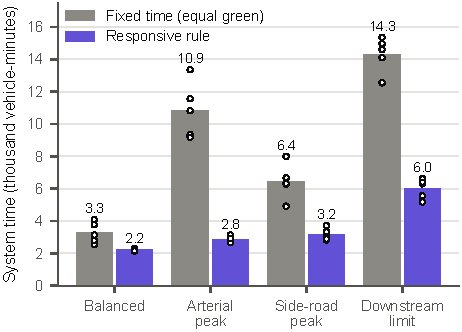
\includegraphics[width=\columnwidth]{control_bars.pdf}
\caption{System time per scenario. Bars are five-seed means; circles are the individual seeds.}\label{fig:bars}
\end{figure}

\begin{figure*}[t]\centering
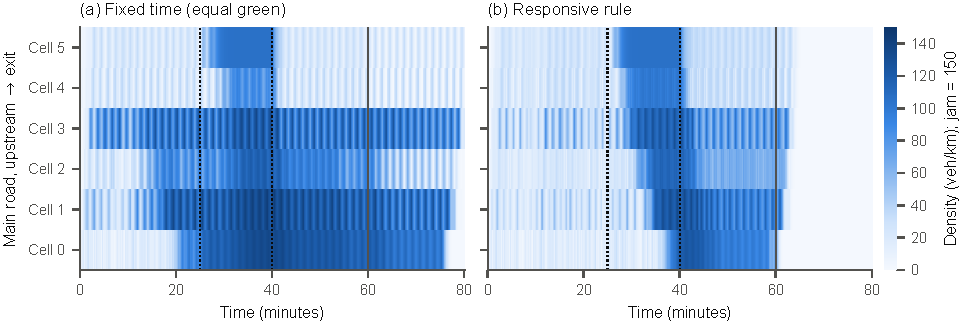
\includegraphics[width=\textwidth]{control_density.pdf}
\caption{Density on the six main cells in the downstream-limit scenario, seed 101. Dotted lines bound the interval of reduced exit capacity; the solid line marks the end of arrivals. Under fixed time the queue reaches the first cell and has not cleared by the end; the responsive rule empties the corridor soon after arrivals stop.}\label{fig:density}
\end{figure*}

The responsive rule gave lower system time in all 20 pairs (Table~\ref{tab:control}, Fig.~\ref{fig:bars}), with mean reductions between 30\% and 74\%. The size of the gap says more about the baseline than about the rule. Each fixed-time approach has green for 8 of 18 steps and can pass at most $2250\times8/18=1000$\,veh/h. The arterial peak sends 1100\,veh/h down the main road, so the fixed plan is over capacity and its queue grows until demand stops. A fixed plan with a longer main green would do much better; ours was not optimised for demand.

Fig.~\ref{fig:density} shows spillback in the downstream-limit scenario. Neither policy can remove a bottleneck at the exit. The fixed plan still held 4.06 vehicles on average at the end of that scenario, which the accounting keeps. Across the 40 runs the largest vehicle-conservation error was $3.0\times10^{-12}$ vehicles and the highest density was 143.6\,veh/km, below jam density.

\subsection{What this experiment shows}
It demonstrates LWR conservation, spillback and two interacting local controllers on a toy corridor. It does not show a benefit in a real city, an optimal controller, multi-agent reinforcement learning, or control driven by the GAT forecasts.

\section{Technical Validation}
\textbf{Protocol integrity.} The experiment protocol and configuration were recorded before real-data training. Run manifests store hashes of source, data and configuration, the sensor order and the normalisation constants. Every method is scored on the same targets and masks, and the re-scored Phase 1 predictions reproduce all 720 recorded metric rows.

\textbf{Tests.} The repository has 76 automated tests. They cover causal windows, training-only statistics, masks, graph direction, tensor shapes, gradient flow, checkpoint and CSV inference, and, for the simulation, the CFL check, red gating, spillback, conservation, state bounds, signal timing and deterministic replay. A fresh run on the merged repository on 18 November 2026 passed all 76 with the raw data present and no skips. The GitHub Actions workflow passed on the canonical main branch on 17 November 2026 with 65 tests passed and 11 skipped, because the dataset is not published to CI.

\textbf{Reproduction.} All eleven evaluated checkpoints reproduce their predictions exactly after reloading. The 40-run simulation is deterministic: independent re-runs on 16 and 17 November reproduced the frozen metric files byte for byte and all 40 trajectory hashes.

\textbf{A recorded deviation.} Memory pressure on the training machine forced one storage change during the study: history windows are built per batch and no longer cached. All 34,249 eligible windows were compared and are bit-identical, and the fitted statistics did not change. Five finished fits were kept and one unfinished fit was restarted from its seed. The lineage is in the evidence folder.

\section{Limitations}
\begin{itemize}
\item \emph{Exposed test interval.} The test interval was inspected in Phase 1, so every forecasting score here is exploratory and not an untouched hold-out estimate.
\item \emph{Deep learning did not win.} The neural models are behind the tree baselines, and behind the historical average at long horizons. The architecture is small, tuning was limited to two learning rates, and the history is 55 minutes.
\item \emph{Narrow evidence for two ablations.} The uniform-weight and no-dropout controls have one seed each.
\item \emph{One network, one season.} Results cover one region and four months. The time zone of the timestamps is unknown, which affects the peak-period split.
\item \emph{Attention is not causation.} Attention weights and per-sensor gains describe the fitted model, not physical influence between roads \cite{attn}.
\item \emph{Synthetic control.} The simulation has assumed parameters, a tiny network, no turning, lane or pedestrian model, and an unoptimised baseline. It is not connected to the forecasts.
\item \emph{Scope.} No project-specific technical brief beyond the general course instructions was available, so the split between forecasting and simulation is our own reading of the project title.
\end{itemize}

\section{Conclusion}
Giving a small recurrent forecaster access to road-graph neighbours through one attention layer lowered its 60-minute MAE from 4.931 to 4.881\,mph, consistently over three seeds and increasingly with horizon. A matched self-loop control shows that the gain comes from the neighbours and not from the extra parameters. The gain is about 1\%, most of it is available from an unweighted neighbour average, and it does not close the 1\,mph gap to the Phase 1 XGBoost baseline. The validation-selected blend is pure XGBoost. For this dataset and this model size, a per-sensor tree model on simple causal features is the better forecaster.

The separate cell-transmission simulation conserves vehicles to numerical precision and shows two local rule-based agents outperforming an equal-green fixed plan in four synthetic scenarios, mainly because that plan is under capacity for the main road.

The most useful next steps are to give the network sensor-specific inputs and a longer history, to evaluate on a new and untouched test period, and, if density or flow data become available, to calibrate the simulation and test whether forecasts can inform the signal agents.

\section*{Contributions and Assistance}
Kavya Katal coordinated preparation and integration. The Phase 2 source code, experiments and evidence were prepared under that coordination with substantial AI assistance, on top of the teammate prototype and the Phase 1 work. Team members integrated and reviewed assigned packages through pull requests: Rudraksh Sharma (synthetic LWR and signal agents), Vridhi Chaudhary (neural preprocessing), Anshuman Mehta (report artefacts and literature), Bineet Keshari (neural models and ablations) and Kavya Katal (evaluation and integration). These review assignments do not establish independent implementation. This report was drafted with AI assistance from the frozen evidence files; its tables and figures are generated by a script from those files. The code and evidence are at \url{https://github.com/KatalKavya96/DLML_Midsem_Project}.

\begin{thebibliography}{00}
\bibitem{cho} K. Cho, B. van Merri\"enboer, C. Gulcehre, D. Bahdanau, F. Bougares, H. Schwenk, and Y. Bengio, ``Learning phrase representations using RNN encoder--decoder for statistical machine translation,'' in \emph{Proc. Conf. Empirical Methods Natural Lang. Process. (EMNLP)}, 2014. [Online]. Available: \url{https://arxiv.org/abs/1406.1078}
\bibitem{pascanu} R. Pascanu, T. Mikolov, and Y. Bengio, ``On the difficulty of training recurrent neural networks,'' in \emph{Proc. 30th Int. Conf. Mach. Learn. (ICML)}, 2013, pp. 1310--1318.
\bibitem{gat} P. Veli\v{c}kovi\'c, G. Cucurull, A. Casanova, A. Romero, P. Li\`o, and Y. Bengio, ``Graph attention networks,'' in \emph{Proc. Int. Conf. Learn. Represent. (ICLR)}, 2018. [Online]. Available: \url{https://arxiv.org/abs/1710.10903}
\bibitem{attn} S. Jain and B. C. Wallace, ``Attention is not explanation,'' in \emph{Proc. Conf. North Amer. Chapter Assoc. Comput. Linguistics (NAACL)}, 2019. [Online]. Available: \url{https://arxiv.org/abs/1902.10186}
\bibitem{dcrnn} Y. Li, R. Yu, C. Shahabi, and Y. Liu, ``Diffusion convolutional recurrent neural network: Data-driven traffic forecasting,'' in \emph{Proc. Int. Conf. Learn. Represent. (ICLR)}, 2018. [Online]. Available: \url{https://arxiv.org/abs/1707.01926}
\bibitem{stgcn} B. Yu, H. Yin, and Z. Zhu, ``Spatio-temporal graph convolutional networks: A deep learning framework for traffic forecasting,'' in \emph{Proc. 27th Int. Joint Conf. Artif. Intell. (IJCAI)}, 2018, pp. 3634--3640, doi: 10.24963/ijcai.2018/505.
\bibitem{gwn} Z. Wu, S. Pan, G. Long, J. Jiang, and C. Zhang, ``Graph WaveNet for deep spatial-temporal graph modeling,'' in \emph{Proc. 28th Int. Joint Conf. Artif. Intell. (IJCAI)}, 2019, pp. 1907--1913, doi: 10.24963/ijcai.2019/264.
\bibitem{lw} M. J. Lighthill and G. B. Whitham, ``On kinematic waves II. A theory of traffic flow on long crowded roads,'' \emph{Proc. Roy. Soc. London A}, vol. 229, no. 1178, pp. 317--345, 1955, doi: 10.1098/rspa.1955.0089.
\bibitem{richards} P. I. Richards, ``Shock waves on the highway,'' \emph{Oper. Res.}, vol. 4, no. 1, pp. 42--51, 1956, doi: 10.1287/opre.4.1.42.
\bibitem{ctm1} C. F. Daganzo, ``The cell transmission model: A dynamic representation of highway traffic consistent with the hydrodynamic theory,'' \emph{Transp. Res. Part B}, vol. 28, no. 4, pp. 269--287, 1994, doi: 10.1016/0191-2615(94)90002-7.
\bibitem{ctm2} C. F. Daganzo, ``The cell transmission model, part II: Network traffic,'' \emph{Transp. Res. Part B}, vol. 29, no. 2, pp. 79--93, 1995, doi: 10.1016/0191-2615(94)00022-R.
\bibitem{ctmoverview} A. D. Patire \emph{et al.}, ``Technical overview of the cell transmission model (CTM),'' Connected Corridors I-210 Pilot, California PATH, Univ. California, Berkeley, Jul. 2015. [Online]. Available: \url{https://connected-corridors.berkeley.edu/sites/default/files/ctm_technical_overview.pdf}
\bibitem{maxpressure} P. Varaiya, ``Max pressure control of a network of signalized intersections,'' \emph{Transp. Res. Part C}, vol. 36, pp. 177--195, 2013, doi: 10.1016/j.trc.2013.08.014.
\bibitem{lioris} J. Lioris and P. Varaiya, ``Variants of max pressure control for a network of signalized intersections,'' working paper, Univ. California, Berkeley, 2013. [Online]. Available: \url{https://connected-corridors.berkeley.edu/sites/default/files/Variants%20of%20Max%20Pressure%20Control%20for%20Signalized%20Intersections.pdf}
\bibitem{rf} L. Breiman, ``Random forests,'' \emph{Mach. Learn.}, vol. 45, no. 1, pp. 5--32, 2001, doi: 10.1023/A:1010933404324.
\bibitem{xgb} T. Chen and C. Guestrin, ``XGBoost: A scalable tree boosting system,'' in \emph{Proc. 22nd ACM SIGKDD Int. Conf. Knowl. Discovery Data Mining}, 2016, pp. 785--794, doi: 10.1145/2939672.2939785.
\bibitem{torchgru} PyTorch Contributors, ``torch.nn.GRU,'' PyTorch 2.7 documentation. [Online]. Available: \url{https://docs.pytorch.org/docs/2.7/generated/torch.nn.GRU.html}
\bibitem{adam} D. P. Kingma and J. Ba, ``Adam: A method for stochastic optimization,'' in \emph{Proc. Int. Conf. Learn. Represent. (ICLR)}, 2015. [Online]. Available: \url{https://arxiv.org/abs/1412.6980}
\bibitem{dropout} N. Srivastava, G. Hinton, A. Krizhevsky, I. Sutskever, and R. Salakhutdinov, ``Dropout: A simple way to prevent neural networks from overfitting,'' \emph{J. Mach. Learn. Res.}, vol. 15, no. 56, pp. 1929--1958, 2014.
\end{thebibliography}
\end{document}
